\documentclass[conference]{IEEEtran}

\usepackage[T1]{fontenc}
\usepackage[utf8]{inputenc}
\usepackage{cite}
\usepackage{amsmath}
\usepackage{graphicx}
\usepackage{booktabs}
\usepackage{array}
\usepackage{multirow}
\usepackage{url}
\usepackage{xurl}
\usepackage[hidelinks]{hyperref}
\usepackage{xcolor}
\usepackage{balance}

\urlstyle{same}

\setlength{\textfloatsep}{9pt plus 2pt minus 2pt}
\setlength{\floatsep}{8pt plus 2pt minus 2pt}
\setlength{\intextsep}{8pt plus 2pt minus 2pt}
\setlength{\abovecaptionskip}{5pt}
\setlength{\belowcaptionskip}{2pt}

\graphicspath{{./}{figures/}{outputs/figures/}}

\newcolumntype{L}[1]{>{\raggedright\arraybackslash}p{#1}}
\newcolumntype{C}[1]{>{\centering\arraybackslash}p{#1}}

\title{FireRoute: Hydrant-Aware Emergency Routing and Dispatch for Campus Fire Response}


\author{
\IEEEauthorblockN{
Kittisak Srimek\IEEEauthorrefmark{1}, and
Kundjanasith Thonglek\IEEEauthorrefmark{1}}
\IEEEauthorblockA{\IEEEauthorrefmark{1}Department of Computer Engineering, Faculty of Engineering, Kasetsart University,
Bangkok, Thailand \\ Email: \{kittisak.srime,kundjanasith.th\}@ku.th}}


\raggedbottom

\begin{document}
\maketitle


\begin{abstract}
Effective fire response requires more than shortest-path routing; it demands the integration of infrastructure constraints, environmental conditions, resource availability, and operational accountability within a unified decision-support process. Existing emergency routing approaches typically optimize travel time in isolation and lack mechanisms for explainable decision-making and post-incident governance. We present \textit{FireRoute}, a hydrant-aware emergency routing and dispatch service that models fire response as a service-level workflow rather than a standalone optimization problem. The proposed system integrates incident intake, explainable risk assessment, risk-weighted routing, hydrant-aware dispatch, responder assignment, and evidence-ready governance into a coherent architecture. A key contribution is a risk-weighted routing model that incorporates access constraints, environmental sensing, and infrastructure status, enabling operationally meaningful route selection. In addition, a hydrant-aware dispatch formulation minimizes responder--hydrant--incident travel cost under asset availability constraints, while an explainable scoring mechanism enhances operator trust in high-stakes scenarios. Scenario-based evaluation on a campus-scale testbed demonstrates that the system adapts to dynamic operational conditions. Results show that smoke exposure can increase route cost by up to 24.0\% and alter hydrant selection, while structural constraints such as alleys introduce moderate cost variations. Furthermore, the system effectively exposes network fragility under blocked conditions and supports transparent interpretation of incident priority.


\end{abstract}


\begin{IEEEkeywords}
Big data services, Decision support service, Emergency response systems,  Explainable artificial intelligence, Hydrant-aware dispatch,  Risk-aware routing
\end{IEEEkeywords}

\section{Introduction}~\label{sec:introduction}
Emergency response operations rarely unfold under stable or fully observable conditions. Dispatchers must make rapid decisions under time pressure, incomplete situational awareness, and dynamically evolving constraints while responders are already en route~\cite{alvear2013}. In such environments, routing, responder allocation, infrastructure readiness, and environmental context cannot be treated as independent components; instead, they must be jointly reasoned in real time to produce actionable and reliable decisions \cite{zografos2002}. Despite advances in intelligent transportation and navigation systems, most existing routing approaches remain fundamentally optimized for nominal travel time, overlooking operational factors such as access limitations, infrastructure availability, and environmental degradation~\cite{jesus2024}. As a result, routes that are computationally optimal may be operationally infeasible or unsafe in real-world emergency scenarios, particularly under dynamic and uncertain conditions.

The increasing availability of Internet of Things (IoT) sensing, distributed infrastructure data, and urban analytics has expanded the potential for data-driven emergency decision support in smart-city environments \cite{asensio2015}. However, integrating these heterogeneous data sources into a unified and operationally meaningful decision-support workflow remains a significant challenge~\cite{park2018}. In practice, emergency vehicle routing is highly sensitive to real-world constraints, including narrow access corridors, gated segments, one-way restrictions, and degraded visibility due to smoke or environmental hazards~\cite{hong2023}. These factors fundamentally alter route feasibility and safety, yet they are often underrepresented or entirely absent in conventional routing formulations \cite{shaaban2019}. As a result, shortest-path solutions may be computationally optimal but operationally impractical~\cite{zhen2024}.

University campuses provide a compelling microcosm of these challenges. Although smaller than urban road networks, campuses exhibit dense, heterogeneous layouts composed of internal roads, service alleys, pedestrian pathways, and restricted-access zones~\cite{sun2024}. In fire response scenarios, the geometrically shortest route is not necessarily the most actionable one. Dispatchers must consider whether routes are traversable by fire vehicles, whether hydrants along the path are operational, and whether environmental conditions compromise maneuverability. Recent work on urban accessibility further emphasizes that operational reachability should be modeled explicitly rather than approximated solely through geometric distance \cite{baik2025}. These observations motivate a shift from purely geometric routing toward operationally decision-support systems.

Despite substantial progress in emergency decision-support systems, three key limitations remain~\cite{sarkar2022}. First, routing is typically treated as an isolated optimization problem, without explicit integration of infrastructure readiness, environmental sensing, and responder state. Second, many systems lack explainability, limiting operator trust and interpretability in high-stakes decision-making scenarios. Third, post-incident accountability and governance are rarely incorporated into system design, resulting in fragmented workflows between dispatch, monitoring, and audit processes. Addressing these limitations requires rethinking emergency routing as part of a broader service-level architecture rather than a standalone algorithmic task. This shift motivates the need for  reproducible systems that can support both real-time decision-making and post-incident analysis within a unified framework.

We present \textit{FireRoute}, a campus-scale emergency routing and dispatch service developed and evaluated on a reproducible pilot testbed around Kasetsart University (Bangkhen). Rather than focusing solely on route optimization, FireRoute frames emergency response as an integrated decision-support workflow that unifies incident intake, explainable risk assessment, risk-weighted routing, hydrant-aware dispatch, responder assignment, and evidence-ready governance. From a big-data service perspective, the system emphasizes the integration of heterogeneous operational data including road constraints, hydrant status, environmental sensing, responder availability, incident descriptors, and audit records into a coherent and inspectable pipeline. The contributions of this paper are as follows:

\begin{enumerate}
    \item We propose a service-oriented formulation of emergency response that integrates routing, environmental sensing, and governance into a decision-support workflow.

    \item We introduce a risk-aware routing and dispatch framework that jointly considers access constraints, infrastructure availability, and environmental conditions, including a hydrant-aware dispatch mechanism that optimizes responder--hydrant--incident chains.

    \item We develop an explainable incident-priority model that exposes interpretable factors influencing dispatch decisions, enabling transparent and trustworthy operation in high-stakes scenarios.

    \item We provide a reproducible system package that externalizes asset, scenario, and governance data, enabling transparent evaluation and reuse for future research.
\end{enumerate}

The remainder of this paper is organized as follows. Section~\ref{sec:background} reviews related work and situates FireRoute within emergency decision-support systems, smart-city sensing, and routing under uncertainty. Section~\ref{sec:methodology} presents FireRoute, including its architecture, data model, and core decision-support mechanisms. Section~\ref{sec:evaluation} describes the evaluation setup, named scenarios, and scenario-based results. Finally, Section~\ref{sec:conclusion} concludes the paper by summarizing the main findings, limitations, and future directions. An unnumbered reproducibility section then summarizes artifact availability and points readers to the detailed execution instructions in the accompanying package.
\section{RELATED WORK}~\label{sec:background}
This section reviews research on emergency decision-support systems, smart-city sensing, and emergency vehicle routing in the context of fire response. Although prior work has improved situational awareness and routing efficiency, these approaches are often developed in isolation and lack integration of heterogeneous data, explainability, and governance. This section highlights these gaps and motivates the design of the proposed FireRoute system.

\subsection{Emergency decision-support systems and incident logistics}
Decision-support systems (DSS) for emergency logistics have long focused on supporting rapid decision-making under time pressure and uncertainty~\cite{su142013423}. Prior systems emphasize integrating traffic conditions, incident reports, and operational constraints to improve response efficiency. A common theme in this body of work is the recognition that effective emergency response requires more than shortest-path computation.


However, existing approaches typically treat routing and decision support as loosely coupled components. While they incorporate elements such as traffic dynamics or incident severity, they often do not jointly model infrastructure readiness (e.g., hydrant availability), environmental sensing, and post-incident accountability within a unified workflow~\cite{fi17120574}. As a result, these systems provide partial decision support but fall short of delivering a fully integrated operational pipeline.

\subsection{Smart-city sensing and fire/disaster systems}
Advances in smart-city infrastructure have introduced a wide range of sensing technologies, including IoT-based environmental monitoring, embedded signaling systems, and building-scale safety platforms~\cite{REJEB2022100565}. These systems demonstrate the potential of real-time data to enhance situational awareness during fire and disaster events. In particular, recent work has highlighted the importance of integrating heterogeneous sensor streams and ensuring system reliability in dynamic and uncertain environments~\cite{SUN2026114440}.

Despite these advances, most sensing-driven systems are designed as monitoring or alerting platforms rather than as decision-support engines. Sensor data is frequently presented through dashboards or visualization interfaces, leaving the burden of interpretation and action on human operators~\cite{NAYAK2024783}. The lack of tight integration between sensing layers and routing or dispatch logic limits the operational impact of these systems, as environmental context is not systematically incorporated into decision-making processes.

\subsection{Emergency vehicle routing and dispatch under uncertainty}
The literature on emergency vehicle routing has explored a variety of optimization strategies, including dynamic routing, traffic-aware path planning, and resource allocation under uncertainty. These approaches have improved routing efficiency and responsiveness, particularly in complex urban environments where congestion and stochastic travel conditions play a significant role.

Nevertheless, most routing models remain focused on optimizing travel time or coverage metrics, with limited consideration of infrastructure constraints and environmental degradation. Additionally, routing and dispatch are often treated as separate problems, leading to fragmented solutions that do not capture the full operational chain from responder deployment to incident resolution~\cite{OLADIGBOLU2025118419}. As a consequence, routing outputs may be mathematically optimal but operationally impractical when real-world constraints such as access limitations or asset availability are taken into account.

\subsection{Positioning of FireRoute}

\begin{figure*}[t]
    \centering
    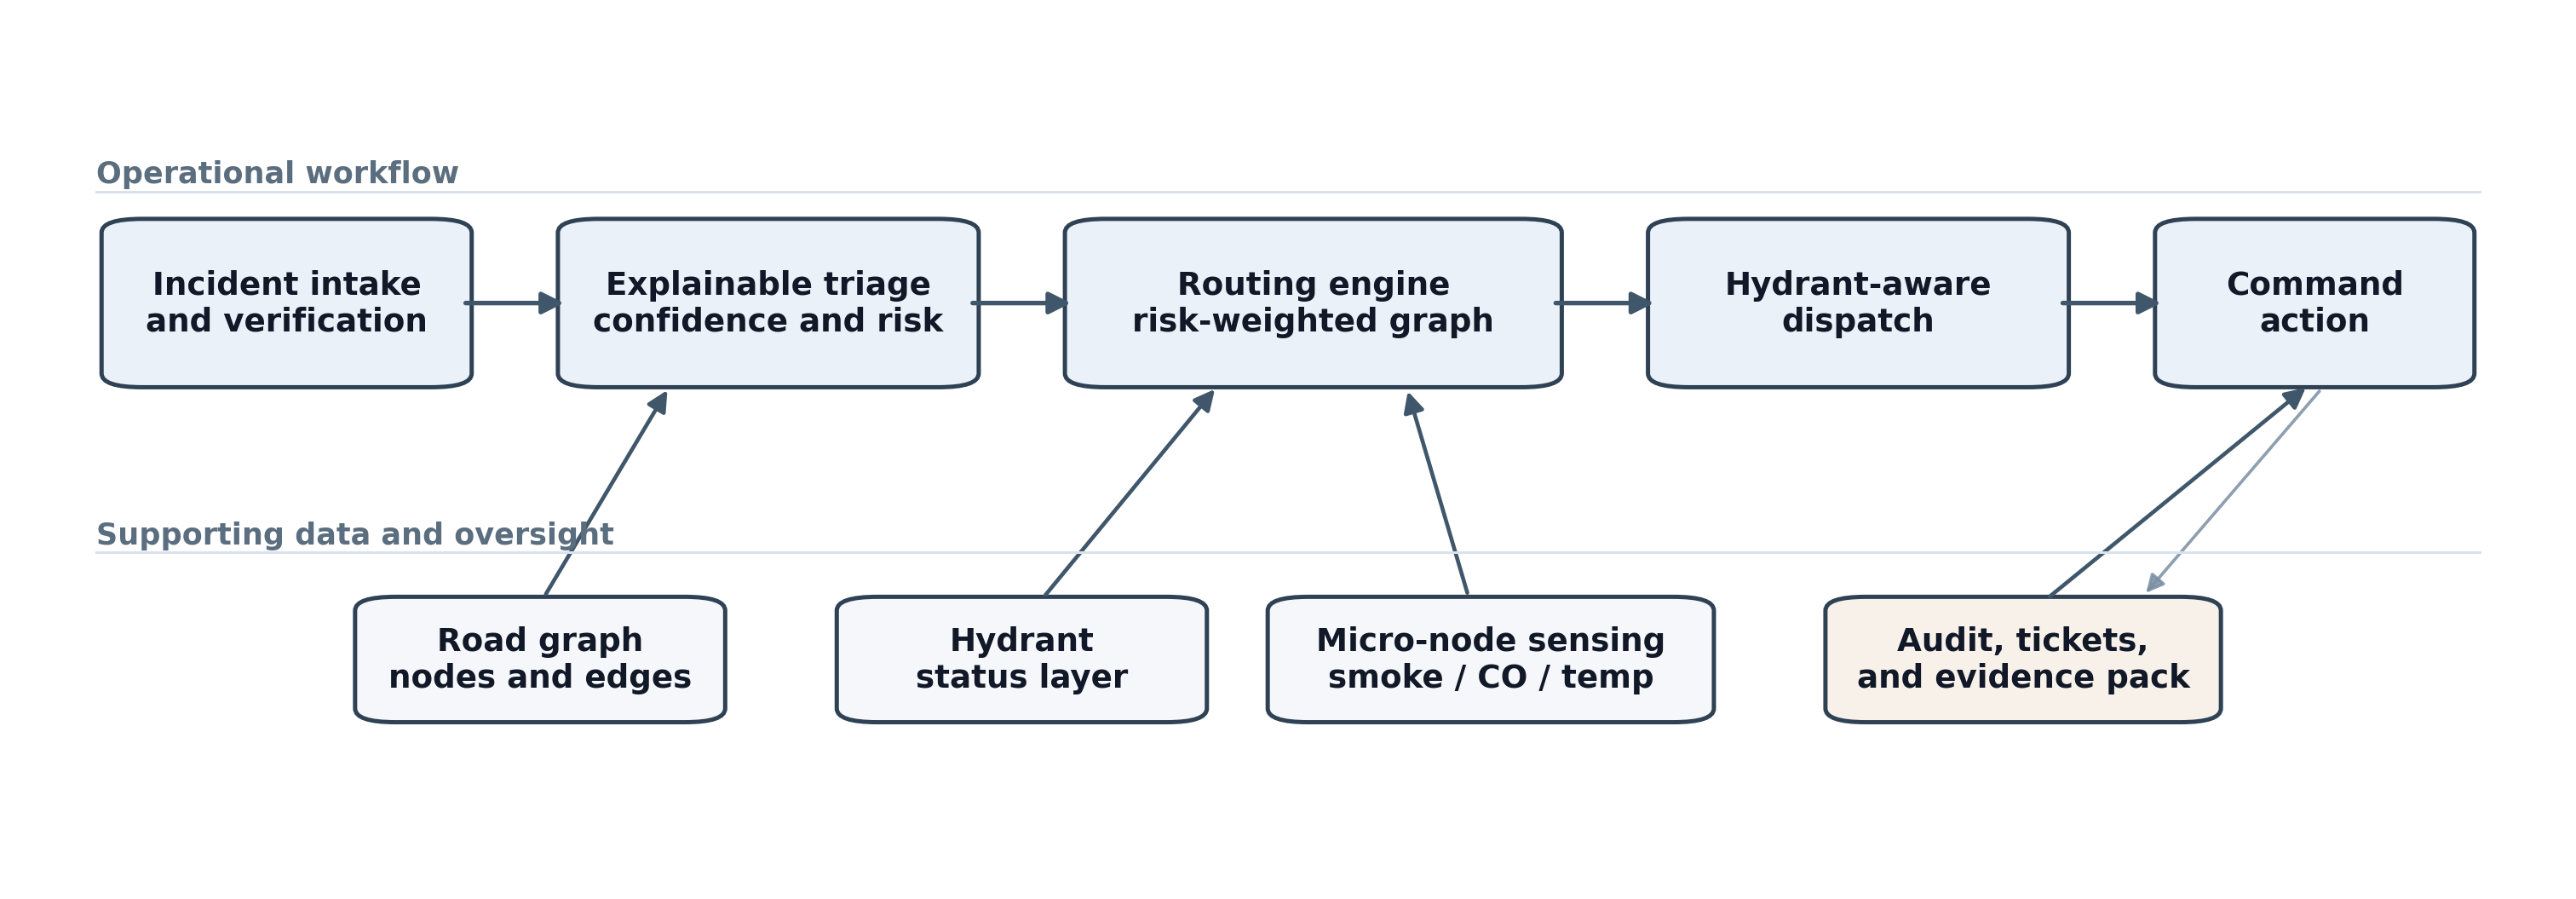
\includegraphics[width=\textwidth]{figure1_architecture}
    \caption{FireRoute architecture integrating incident intake, explainable triage, risk-weighted routing, hydrant-aware dispatch, and evidence-ready governance.}
    \label{fig:architecture}
\end{figure*}

In contrast to prior work, FireRoute is designed as an integrated, service-level decision-support system rather than a routing-only solution. The key distinction lies in its holistic treatment of emergency response as a workflow that connects incident intake, explainable risk assessment, risk-aware routing, hydrant availability, environmental sensing, dispatch actions, and governance outputs within a single architecture.

Rather than optimizing routing in isolation, the system emphasizes operational realism, explainability, and reproducibility. This positioning aligns with emerging directions in intelligent urban systems, where decision support is expected to combine heterogeneous data sources, support human interpretability, and enable accountability through auditable system outputs. By bridging routing, sensing, and governance within a unified framework, FireRoute advances beyond traditional approaches and provides a foundation for next-generation emergency response systems.
\section{FireRoute}~\label{sec:methodology}
This section presents the proposed FireRoute framework, which models emergency response as an integrated, service-level decision-support system. Unlike conventional approaches that treat routing as an isolated optimization problem, FireRoute unifies incident intake, risk assessment, routing, dispatch, and governance within a single operational workflow. The methodology is designed to incorporate heterogeneous data sources, support explainable decision-making, and enable reproducibility through structured data.


\subsection{System Architecture}

FireRoute system is organized into six interconnected layers: (i) incident intake, (ii) explainable triage, (iii) risk-weighted routing, (iv) hydrant-aware dispatch, (v) command and control actions, and (vi) evidence-ready governance. These layers operate on top of shared data abstractions, including graph, asset, sensor, incident, and governance layers, forming a unified pipeline from data ingestion to decision output.


Our key design principle is to move beyond path computation and instead support a dispatch-relevant workflow that can be interpreted in real time and audited post hoc. Figure~\ref{fig:architecture} illustrates the interaction between these components, highlighting the integration of routing logic with environmental sensing, infrastructure state, and operational decision-making.

\subsection{Data Model and Integration}

The system operates on multiple heterogeneous data layers. The graph layer models the road network as a structured graph with attributes such as edge width, turn radius, and access constraints. The asset layer includes hydrants and responders, capturing operational states such as availability and functionality~\cite{P2026108912}. The sensor layer provides environmental measurements, including smoke, carbon monoxide, and temperature. The incident layer stores structured descriptors of reported events, while the governance layer records audit logs, maintenance tickets, and evidence artifacts.

To ensure transparency and reproducibility, all data components are externalized as structured CSV and JSON files. This design enables routing and dispatch outcomes to be directly traced to input configurations, supporting controlled experimentation, scenario replay, and systematic validation of system behavior. Furthermore, it facilitates independent verification and extension of the system by other researchers without requiring access to the original implementation.

\subsection{Operational Workflow}

The FireRoute workflow begins with incident intake, where operators input structured information such as location, trapped-person count, fuel type, panic indicators, and access conditions. Based on these inputs and environmental sensor data, the system computes an explainable risk score and a dispatch-confidence estimate.

Following triage, the operator can generate either a direct route or a hydrant-aware route. The system then assigns an appropriate responder based on availability and estimated travel cost. Throughout this process, infrastructure conditions (e.g., hydrant status) and environmental factors (e.g., smoke levels) are incorporated into decision-making. Finally, all actions and results are recorded in the governance layer, enabling post-incident review and accountability.

\subsection{Risk-Weighted Routing Model}

The road network is modeled as a graph $G=(V,E)$, where routing is performed using Dijkstra’s algorithm over an operational cost function. The baseline traversal time of an edge $e$ is defined as
\begin{equation}
\tau(e) = \frac{d(e)}{v(e)},
\end{equation}
where $d(e)$ is the geographic distance and $v(e)$ is the nominal traversal speed.

To capture real-world constraints, FireRoute introduces a risk-weighted cost function:
\begin{equation}
C(e) = \tau(e)\,\kappa(e),
\end{equation}
where $\kappa(e)$ is an operational penalty multiplier. For blocked edges, infeasibility is enforced through
\begin{equation}
\kappa(e) = 10^9.
\end{equation}
Otherwise, the penalty is defined as
\begin{equation}
\kappa(e) = (1 + 0.25A\alpha)(1 + 0.20G)(1 + 0.05O)(1 + 0.30\sigma),
\end{equation}
where $A$ indicates alley segments, $\alpha$ is the alley severity factor, $G$ represents gate constraints, $O$ denotes one-way restrictions, and $\sigma$ captures environmental degradation (e.g., smoke). This formulation enables the routing model to reflect operational feasibility rather than purely geometric optimality.

\subsection{Hydrant-Aware Dispatch}
For fire operations that require water access, routing directly to the incident is not always sufficient. Let $r$ be the responder node, $i$ the incident node, and $H_W$ the set of hydrants currently marked \textit{WORKING}. FireRoute evaluates candidate hydrants using
\begin{equation}
h^\star=\arg\min_{h \in H_W} \left(T(r,h)+T(h,i)\right),
\end{equation}
where $T(x,y)$ is the risk-weighted route cost between nodes $x$ and $y$. Hydrants in other states are excluded from the candidate set. The selected hydrant is therefore not simply the nearest one on the map; it is the one that minimizes the operational chain cost under current conditions.

\subsection{Explainable Risk Modeling}

To enhance operator trust, FireRoute employs a transparent additive model for incident prioritization:
\begin{equation}
R = \operatorname{clip}(20 + 8P + F + A + 10M + E,\; 0,\; 100),
\end{equation}
where $P$ is the number of trapped persons, $F$ represents fuel-related risk, $A$ encodes access difficulty, $M$ indicates panic conditions, and $E$ captures environmental severity derived from sensor data. The use of interpretable components allows operators to understand and validate system recommendations in real time.

\subsection{Dispatch Confidence Estimation}

In addition to risk scoring, the system estimates dispatch confidence as a measure of input completeness and reliability:
\begin{equation}
Q = \operatorname{clip}(0.35 + c_f + m - d_p,\; 0,\; 1).
\end{equation}
where $c_f$ reflects completeness of report fields, $m$ denotes media or panic indicators, and $d_p$ captures duplicate-report penalties. This score provides an auxiliary signal for decision-making under uncertainty.

\subsection{Evidence-Ready Governance}

A distinguishing feature of FireRoute is its integration of governance into the operational workflow. The system records audit events throughout the incident lifecycle, supports maintenance ticket generation for infrastructure assets, and produces an evidence package containing routing results, hydrant states, incident descriptors, and after-action summaries.

This design enables traceability, accountability, and reproducibility, transforming emergency routing from a transient decision process into a verifiable and auditable system.

\subsection{Data Package and Repository Organization}

The FireRoute reproducibility package externalizes the pilot graph, operational assets, scenario controls, and governance seeds into structured CSV/JSON files. This design separates data from application logic and allows routing results, table generation, and evidence artifacts to be reproduced without editing source code. The repository is organized into five main layers: \texttt{app/} for the prototype, \texttt{data/} for graph and asset files, \texttt{scripts/} for reproduction utilities, \texttt{outputs/} for generated artifacts, and \texttt{docs/} for reproducibility guidance. The graph package includes \texttt{nodes.csv} and \texttt{edges.csv}, while hydrants, sensors, and responder states are stored as standalone asset tables. Scenario files encode perturbations such as smoke, alley constraints, and blocked connectors, thereby providing explicit inputs for the evaluation cases reported in the paper.
\section{Evaluation}~\label{sec:evaluation}
This section evaluates the proposed FireRoute system through scenario-based experiments on a controlled campus-scale testbed. The evaluation focuses on how the system responds to operational constraints, environmental perturbations, and infrastructure conditions, as well as its ability to provide interpretable and actionable decision support.

\subsection{Experimental Setup}

\begin{table}[t]
\caption{Pilot package summary for graph, asset, scenario, and governance artifacts.}
\label{tab:assets}
\centering
\scriptsize
\setlength{\tabcolsep}{3.5pt}
\renewcommand{\arraystretch}{0.92}
\begin{tabular}{L{2.25cm} C{0.8cm} L{3.95cm}}
\toprule
Artifact & Count & Notes \\
\midrule
Graph nodes & 21 & Campus stations, road anchors, shelters, and POIs \\
Graph edges & 25 & Main roads, alleys, and footpath connectors \\
Hydrants & 12 & Mixed operational states with health-check metadata \\
Sensors & 3 & Smoke, carbon monoxide, and temperature nodes \\
Responders & 3 & Two available units and one busy unit \\
Named scenarios & 5 & Baseline, smoke, alley, near-station, blocked-edge \\
Governance seeds & 3+ & Demo incidents, status log, and ticket seed file \\
\bottomrule
\end{tabular}
\end{table}

\subsubsection{Pilot graph scope}
The current package uses a deliberately compact yet operationally meaningful pilot graph consisting of 21~nodes, 25~edges, 12~hydrants, 3~sensor nodes, and 3~responder units. Although small in scale, the graph is carefully constructed to preserve key structural and operational characteristics commonly observed in real-world campus environments, including mixed-access road segments, constrained service alleys, gated connectors, and limited redundancy in certain corridors. This level of abstraction allows the graph to remain fully inspectable and interpretable, enabling detailed analysis of routing decisions and system behavior.

At the same time, the graph is sufficiently expressive to capture critical operational factors such as gate restrictions, alley-induced traversal penalties, variability in hydrant availability, and environmental degradation effects derived from sensor inputs. These features enable controlled experimentation on how routing and dispatch decisions respond to infrastructure constraints and dynamic conditions. The inclusion of responder units with distinct spatial locations further allows evaluation of assignment strategies under heterogeneous deployment scenarios. The pilot graph provides a balanced testbed that supports both qualitative interpretation and quantitative analysis of system behavior under realistic yet controlled conditions.


\subsubsection{Scenario definitions}
Five named scenarios are used to examine the system under nominal, degraded, and disrupted conditions. These are \texttt{baseline\_e3}, \texttt{smoke\_e3\_08}, \texttt{alley\_e3\_10}, \texttt{near\_station\_n1}, and \texttt{blocked\_e1\_e2}. Together, they represent baseline routing, environmental degradation, narrow-access penalties, near-station dispatch trade-offs, and corridor blockage. Each scenario is encoded as a structured JSON file specifying the incident location, routing parameters, and any graph modifications such as blocked edges.

\subsubsection{Evaluation questions}
The evaluation is organized around four practical questions:
\begin{enumerate}
    \item \textbf{Sensitivity:} Does route cost respond consistently to smoke, alley, and blockage perturbations?
    \item \textbf{Adaptivity:} Does hydrant selection change appropriately when routing conditions or infrastructure constraints change?
    \item \textbf{Interpretability:} Does the explainable risk score scale in a transparent way with incident severity?
    \item \textbf{Fragility exposure:} Does the system explicitly reveal operational fragility rather than concealing it behind nominal shortest-path output?
\end{enumerate}

\subsubsection{Ablation settings}
The package also supports targeted ablations by disabling specific components of the operational logic. These ablations clarify which prototype behaviors depend on which modeling assumptions, including smoke penalties, alley penalties, hydrant filtering, and blocked-edge infeasibility. This design enables systematic isolation of individual factors, allowing the contribution of each component to be evaluated independently in terms of sensitivity, realism, and decision impact.


\begin{table}[!t]
\caption{Ablation settings used to interpret component-level behavior.}
\label{tab:ablation}
\centering
\scriptsize
\setlength{\tabcolsep}{4pt}
\renewcommand{\arraystretch}{0.96}
\begin{tabular}{L{2.3cm} L{1.8cm} L{3.2cm}}
\toprule
Ablation & Change applied & Expected operational effect \\
\midrule
No smoke penalty & Set smoke factor to 0 & Removes dynamic visibility/risk penalty; routes revert toward baseline travel preference. \\
No alley penalty & Set alley factor to 0 & Reduces sensitivity to narrow-access segments; alley-heavy paths become more competitive. \\
No hydrant filtering & Allow non-\textit{WORKING} hydrants in candidate set & Lowers nominal dispatch cost in some cases but reduces operational plausibility. \\
No blocked-edge infeasibility & Remove extreme blocked-edge penalty & Allows nominal routing through disrupted connectors and suppresses fragility signals. \\
\bottomrule
\end{tabular}
\end{table}

\subsection{Results and Analysis}

\subsubsection{Baseline routing and responder split}
Across the pilot graph, motorbike responder FR-01 at HQ is fastest to 10 of the pilot destinations, while truck TR-07 at the west gate is fastest to the remaining 10. This near-even split indicates that the assignment logic reflects actual responder positioning rather than trivial bias toward a particular unit.

From an operational perspective, this result suggests that the system effectively captures spatial heterogeneity in responder deployment. The balanced distribution also implies that routing decisions are sensitive to geographic layout rather than being dominated by a single responder location. This behavior is important in real-world scenarios, where uneven responder utilization can lead to delayed response times and resource bottlenecks.

\subsubsection{E3 baseline and perturbation results}
For the eastern service-lane incident at node E3, the baseline direct route from FR-01 follows
HQ $\rightarrow$ N1 $\rightarrow$ N2 $\rightarrow$ N3 $\rightarrow$ N4 $\rightarrow$ E1 $\rightarrow$ E2 $\rightarrow$ E3,
with an estimated travel time of 185.5~s. In hydrant-aware mode, the system selects HYD-102, which lies directly along the operational chain, resulting in no additional dispatch overhead. This indicates that the baseline route is already aligned with available infrastructure, allowing efficient integration of water access without requiring detours.


When the smoke factor is increased to 0.8, the direct ETA rises to 230.0~s, representing an increase of approximately 24.0\% relative to the baseline. In addition, the preferred hydrant shifts from HYD-102 to HYD-104. This dual effect demonstrates that environmental degradation not only increases traversal cost but also alters optimal resource selection. In other words, the system responds to degraded conditions by jointly adapting both routing and hydrant selection, rather than treating them independently.

In contrast, increasing the alley factor to 1.0 results in a smaller increase to 198.7~s (approximately 7.1\% above baseline). This comparatively modest change indicates that structural constraints such as narrow-access segments influence routing decisions, but to a lesser degree than dynamic environmental factors such as smoke. This observation highlights the relative importance of environmental conditions in shaping operational feasibility.

\begin{table}[t]
\caption{Scenario-based routing outcomes on the pilot graph.}
\label{tab:scenarios}
\centering
\scriptsize
\setlength{\tabcolsep}{4pt}
\renewcommand{\arraystretch}{0.96}
\begin{tabular}{L{1.55cm} C{0.95cm} C{0.95cm} C{1.0cm} L{2.7cm}}
\toprule
Scenario & Direct ETA (s) & Hydrant & Chain ETA (s) & Operational interpretation \\
\midrule
E3 baseline & 185.5 & HYD-102 & 185.5 & Hydrant lies on-path; no additional dispatch overhead. \\
E3 + smoke 0.8 & 230.0 & HYD-104 & 230.0 & Route cost rises by about 24\%; hydrant preference changes under degraded conditions. \\
E3 + alley 1.0 & 198.7 & HYD-102 & 198.7 & Moderate increase from alley-aware weighting. \\
N1 near station & 34.2 & HYD-102 & 76.6 & Direct dispatch remains preferable when the incident is close to HQ. \\
E3 + blocked E1--E2 & Infeasible & --- & Infeasible & Corridor becomes unreachable, revealing fragility. \\
\bottomrule
\end{tabular}
\end{table}


\subsubsection{Near-station trade-off}
For an incident at node N1, the direct route from HQ requires only 34.2~s, whereas the hydrant-aware plan increases the total travel time to 76.6~s via HYD-102. This scenario reveals an important operational trade-off between minimizing response time and ensuring water accessibility.

The result suggests that hydrant-aware routing should not be enforced uniformly, but rather exposed as a decision option to operators. In time-critical situations, rapid arrival may take precedence over immediate access to water resources, whereas in high-risk fire scenarios, hydrant proximity may become more critical. By explicitly surfacing this trade-off, the system supports informed decision-making rather than enforcing a single optimization objective.


\subsubsection{Fragility under blockage}
Blocking the E1--E2 corridor renders the eastern routing chain operationally infeasible under the current penalty formulation. Instead of rerouting through suboptimal or unsafe alternatives, the system explicitly reports infeasibility. This behavior highlights the system’s ability to prioritize operational safety and realism over forced feasibility.


This behavior is significant because it reveals structural fragility within the network. Rather than masking disruptions through fallback shortest-path solutions, the system exposes critical bottlenecks and single points of failure. From a planning perspective, such insights can inform infrastructure improvements, redundancy design, and contingency planning, making the system valuable not only for real-time response but also for long-term resilience analysis.

\subsubsection{Explainable risk behavior}
The explainable risk model produces outputs that are consistent with operational expectations. A low-severity case near sensor SN-03 yields a score of 27.8, while a more severe case involving trapped individuals, hazardous fuel, and restricted access increases to 73.8.


Under extreme conditions, such as multiple trapped individuals and high-risk fuel types, the score saturates at 100. These scores are not only monotonic with respect to severity but also interpretable in terms of their contributing factors. Operators can directly trace how individual components, such as trapped-person count or environmental conditions, influence the final score. This transparency is essential for trust in high-stakes environments, where black-box predictions may be difficult to justify or validate.


\begin{figure*}[t]
    \centering
    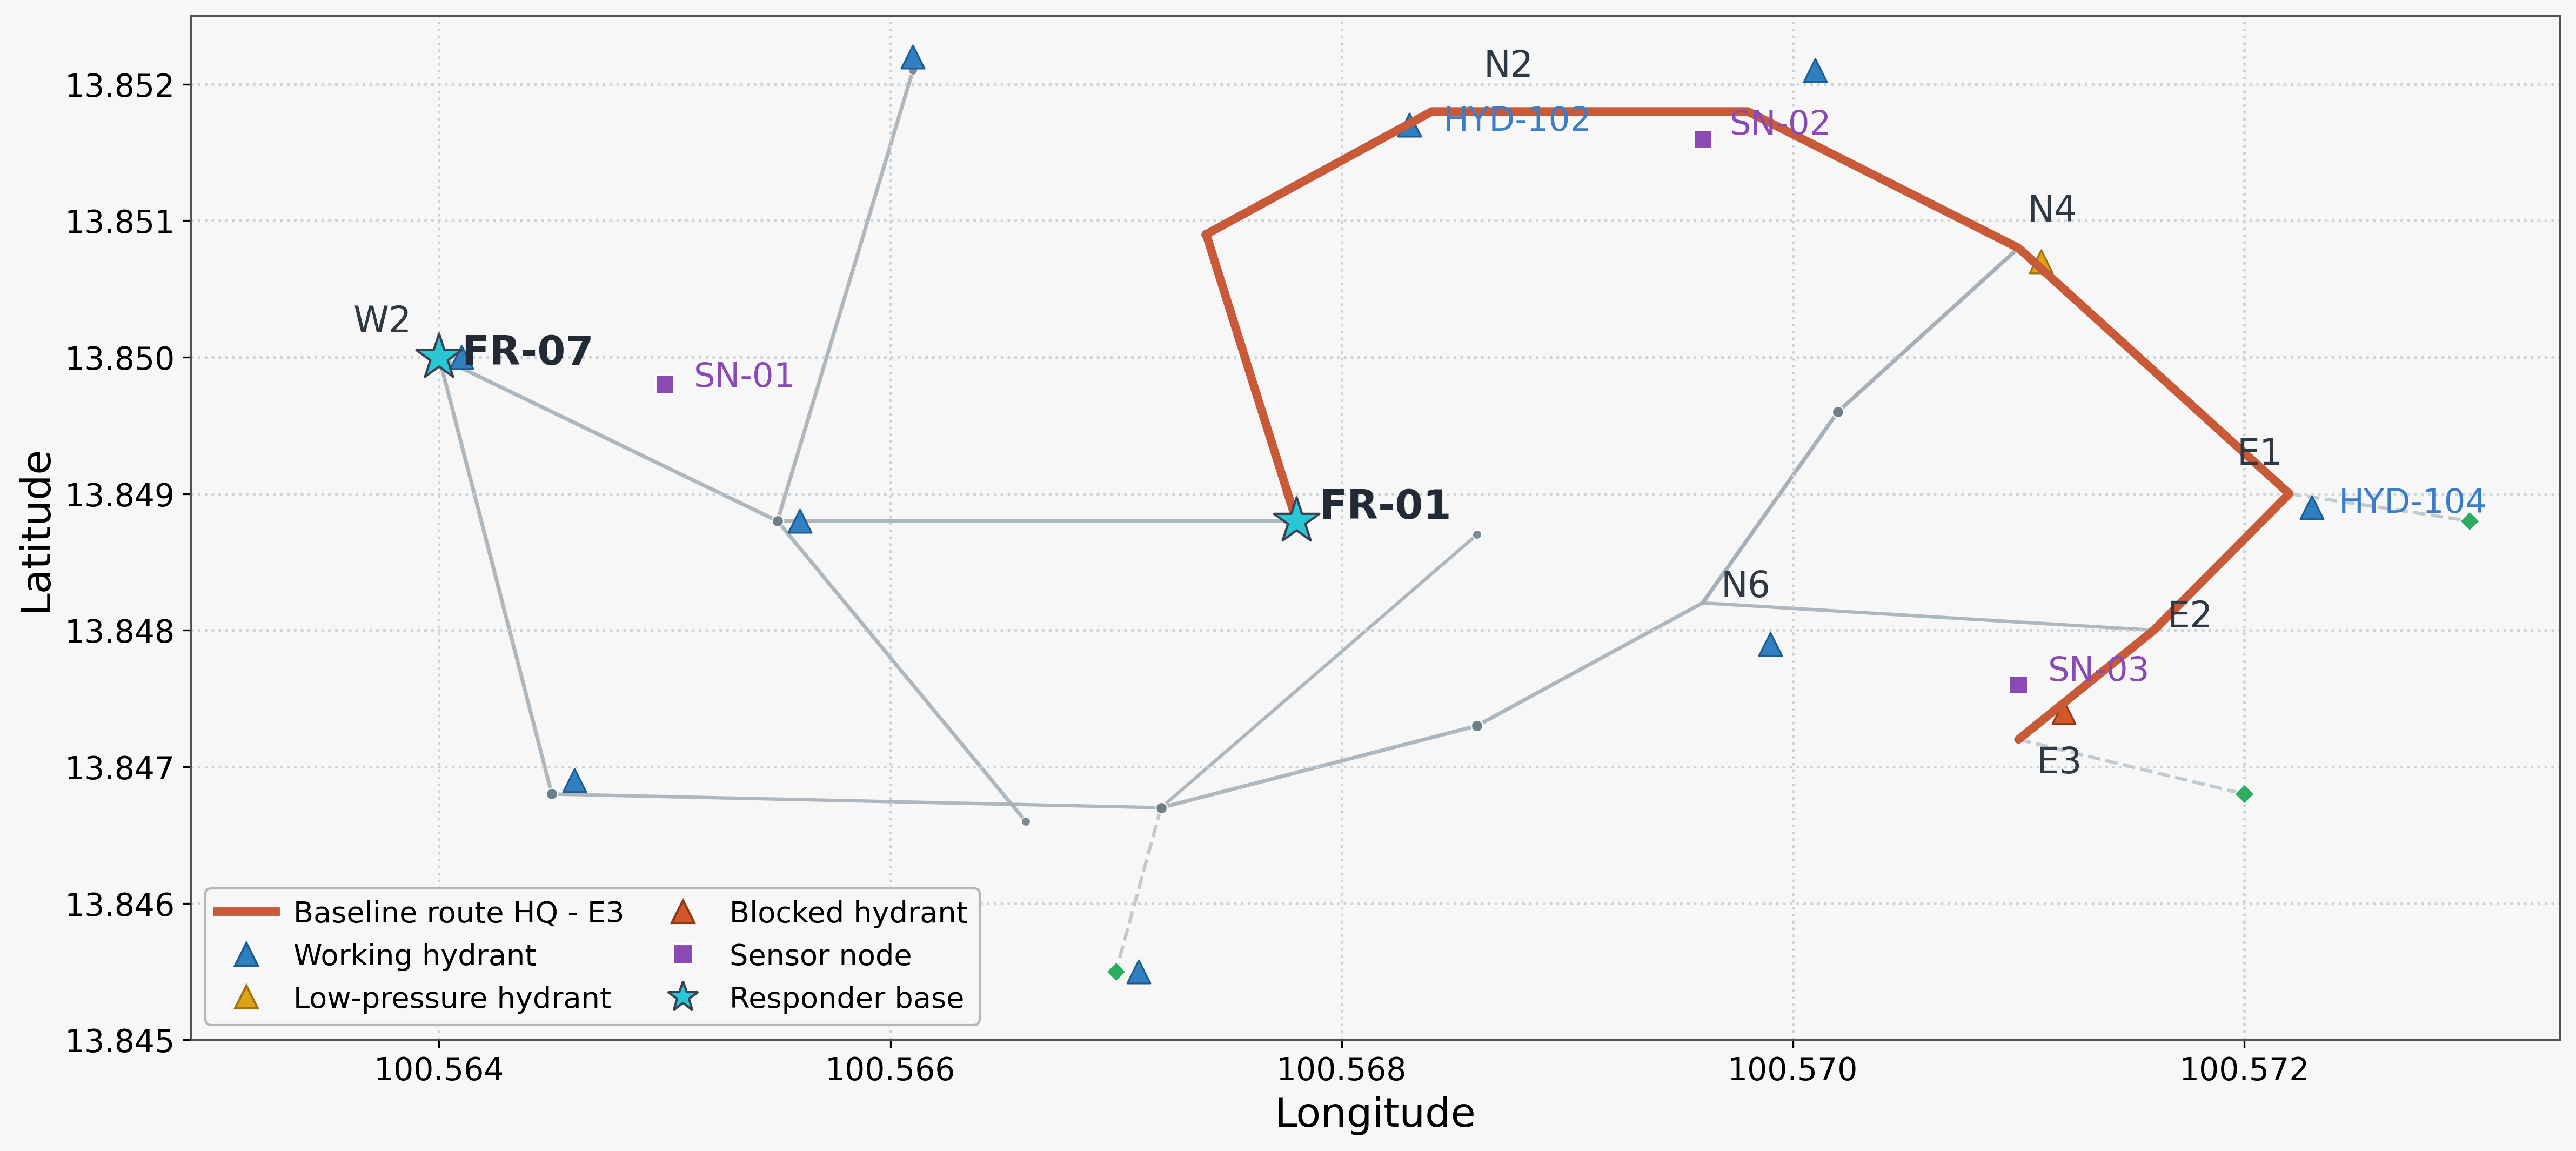
\includegraphics[width=\textwidth]{figure2_pilot_map}
    \caption{Pilot graph and baseline eastern-corridor route reproduced from the package configuration, with hydrants, sensor nodes, and responder bases overlaid from the externalized asset files.}


    \label{fig:pilotmap}
\end{figure*}


\subsubsection{Ablation interpretation}
The ablation study provides detailed insight into the role of each modeling component and its contribution to overall system behavior. By selectively disabling individual factors, we can isolate how specific assumptions influence routing decisions, dispatch outcomes, and system interpretability.

Removing the smoke penalty collapses the difference between the \texttt{smoke\_e3\_08} scenario and the baseline, confirming that environmental degradation acts as a dominant driver of route cost variation. This indicates that the system appropriately captures the impact of dynamic environmental conditions, such as reduced visibility and maneuverability, on operational feasibility. In contrast, removing alley penalties reduces sensitivity to narrow-access constraints, demonstrating that structural factors contribute to routing behavior but exert a comparatively smaller effect than environmental conditions.

Allowing non-\textit{WORKING} hydrants into the candidate set reduces nominal dispatch cost in some scenarios, but leads to operationally unrealistic recommendations. This highlights the importance of infrastructure filtering in ensuring that optimization results remain grounded in real-world feasibility. Similarly, removing blocked-edge infeasibility allows routing through disrupted corridors, effectively suppressing fragility signals and masking critical vulnerabilities in the network. This behavior underscores the importance of explicitly modeling infeasibility to reveal structural weaknesses rather than obscuring them.

Figure~\ref{fig:pilotmap} provides a spatial visualization of the pilot graph and baseline routing behavior. It illustrates how routing decisions interact with the physical layout of the environment, including the placement of hydrants, sensor nodes, and responder bases. This visual representation helps contextualize how constraints such as blocked corridors or narrow access paths influence feasible routes and system behavior. Table~\ref{tab:scenarios} presents a quantitative summary of scenario-based outcomes, including direct travel time, hydrant selection, and overall chain cost. The table highlights how different perturbations systematically affect routing efficiency and resource allocation, making it easier to compare the relative impact of environmental and structural factors across scenarios.

Our ablation results demonstrate that each modeling component contributes meaningfully to system performance. Rather than simply computing shortest paths, the proposed framework encodes operational assumptions that govern sensitivity to environmental conditions, adherence to infrastructure constraints, and interpretability of decision outcomes.


\

\section{Conclusion}~\label{sec:conclusion}
In this paper, we presented FireRoute, a service-oriented emergency routing and dispatch framework that integrates routing, hydrant availability, environmental sensing, and governance into a unified decision-support workflow. Rather than proposing a new shortest-path algorithm, the contribution lies in demonstrating how heterogeneous operational factors can be systematically combined to produce routing and dispatch decisions that are both actionable and interpretable. The results show that the system responds meaningfully to infrastructure constraints, while also exposing structural fragility that is often overlooked in traditional routing approaches.

From a systems perspective, FireRoute illustrates the value of treating emergency response as a data-driven service pipeline rather than a standalone optimization task. By incorporating explainable risk modeling and evidence-ready governance, the framework supports not only real-time decision-making but also post-incident analysis and accountability. The accompanying reproducibility package further strengthens the contribution by enabling transparent evaluation, scenario replay, and independent verification of results.

Despite these contributions, several limitations remain. The current pilot graph is relatively small and relies on approximate spatial representations. The risk and confidence models are heuristic and not yet calibrated against real-world dispatch data. Environmental factors such as smoke and access constraints are controlled through scenario parameters rather than derived from live sensor fusion. Additionally, blocked edges are modeled using an extreme penalty, which effectively reveals fragility but does not yet incorporate adaptive rerouting strategies or redundancy-aware planning.

Our work will focus on extending the framework toward larger-scale and more realistic deployments. This includes expanding the graph to city-scale networks, integrating real-time sensor streams and historical incident data, and learning parameter weights from operational datasets. Further research will explore adaptive routing strategies that balance feasibility and resilience, as well as multi-objective optimization formulations that jointly consider response time, safety, and resource utilization. In addition, incorporating predictive modeling and uncertainty-aware decision-making could enhance system robustness under incomplete or noisy inputs. Ultimately, these directions aim to transform FireRoute from a controlled pilot system into a scalable and deployable solution for real-world emergency response environments.
\section*{Reproducibility and Artifact Availability}
The review artifact package includes the FireRoute prototype source code, externalized graph and asset files, named scenario JSON files, generated output artifacts, and the documentation needed to reproduce the main paper outputs. In particular, the package contains the source code, graph/assets/scenarios data, output files used for scenario-based evaluation, and the accompanying \texttt{README.md} and \texttt{REPRODUCE.md} files. These materials allow the main scenario outcomes reported in this paper to be inspected and replayed from structured inputs rather than narrative description alone. The review artifact package is available at \href{https://drive.google.com/drive/folders/1yWOCC4-r6X0Ld1G7pwZhpD3XnHFCyvn9?usp=sharing}{this link}. Detailed setup and execution instructions are provided in the included \texttt{README.md} and \texttt{REPRODUCE.md} files.


\balance
\bibliographystyle{IEEEtran}
\bibliography{refs}

\end{document}